\label{methodology-chapter}
%\section{End-to-End Security Formalization}
%\label{methodology}

In this chapter, we completely formalize everything
discussed in Section~\ref{informal-methodology}, showing
how security can be soundly propagated from a high-level 
specification to a low-level implementation. Figure~\ref{simulations}
pictures the overall setup. We have many different machine
semantics; the bottom one represents our lowest-level model of 
the actual systems code executing over physical hardware,
while the top semantics represents our highest-level abstraction
of the system, complete with logical state. We connect all
of these semantics together with formal simulations, and
show how the unwinding condition noninterference property
at the highest abstraction level automatically guarantees
an end-to-end, whole-execution noninterference property for
the lowest level.

\begin{figure}
\centering{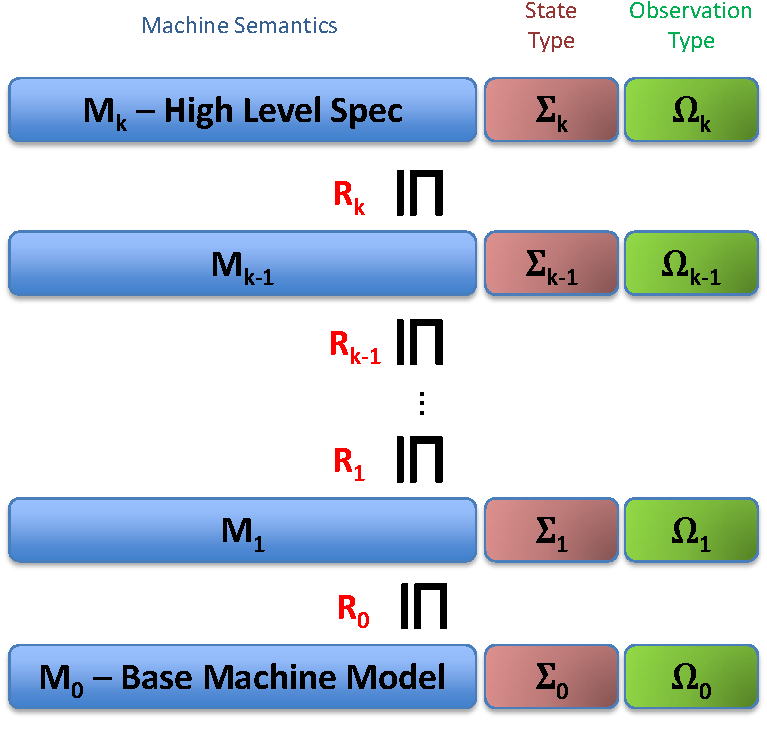
\includegraphics[scale=0.53]{pldi/figure/simulations.pdf}}
\caption{\small{Basic Setup~--- Many simulations are chained together to 
incrementally refine a top-level specification semantics into a
concrete implementation executing over a low-level assembly machine
model.}}
%\vspace*{-2ex}
\label{simulations}
\end{figure}

\section{Machines with Observations}
\label{methodology-machine}

In the following, assume we have a set $\mathcal{P}$ of distinct 
principals or security domains.

\begin{definition}[Machine]
A \emph{state transition machine} $M$ consists 
of the following components (assume all sets may be finite or infinite):
\newpage
\begin{itemize} \itemsep 0pt
\item a type $\Sigma_M$ of program state
\item a set of initial states $I_M$ and final states $F_M$
\item a transition (step) relation $T_M$ of type 
$\pwrset{\Sigma_M \times \Sigma_M}$
\item a type $\Omega_M$ of observations
\item an observation function $\observem{M}{p}{\sigma}$ 
of type $\mathcal{P} \times \Sigma_M \to \Omega_M$
\end{itemize}
\end{definition}

\noindent
When the machine $M$ is clear from context, 
we use the notation $\sigma \steprel \sigma'$ to mean
$(\sigma,\sigma') \in T_M$.
For multiple steps, we define $\sigma \steprel^n \sigma'$ in
the obvious way, meaning that there exists a chain of states
$\sigma_0,...,\sigma_n$ with $\sigma = \sigma_0$, $\sigma' = \sigma_n$,
and $\sigma_i \steprel \sigma_{i+1}$ for all $i \in [0,n)$.
We then define $\sigma \steprel^* \sigma'$ to mean that there exists 
some $n$ such that $\sigma \steprel^n \sigma'$, and
$\sigma \steprel^+ \sigma'$ to mean the same but with a nonzero $n$.

Notice that our definition is a bit different from many traditional
definitions of automata, in that we do not define any explicit notion of 
actions on transitions. In traditional definitions, actions are used
to represent some combination of input events, output events, and
instructions/commands to be executed. In our approach, we advocate moving 
all of these concepts into the program state (which can contain both
concrete and logical state)~--- this simplifies the theory,
proofs, and policy specifications.

\paragraph{Initial States vs Initialized States}
Throughout our formalization, we do not require anything regarding 
initial states of a machine. The reason is related to
how we will actually carry out security and simulation proofs in 
practice (described with respect to the mCertiKOS security proof in
Chapters~\ref{casestudy-def-chapter} and~\ref{casestudy-proof-chapter}). We never 
attempt to reason about the true initial state of a machine; instead,
we assume that some appropriate setup/configuration process brings us from
the true initial state to some properly \emph{initialized} state,
and then we perform all reasoning under the assumption of
proper initialization.

\section{High-Level Security}
\label{methodology-security}
As described in Chapter~\ref{informal-chapter}, we use different notions of
security for the high level and the low level. High-level security says
that each individual step preserves indistinguishability. It also
requires a safety proof as a precondition, guaranteeing that 
the machine preserves some initialization invariant $I$.

\begin{definition}[Safety]
We say that a machine $M$ is safe under state predicate $I$, 
written $\safe{M}{I}$, when the following progress and
preservation properties hold:
{\small\begin{align*}
& 1.) \quad \forall \sigma \in I - F_M \such
\exists \sigma' \such \sigma \steprel \sigma' \\
& 2.) \quad \forall \sigma, \sigma' \such
\sigma \in I \land
\sigma \steprel \sigma' \Longrightarrow \sigma' \in I
\end{align*}}
\end{definition}

\begin{definition}[High-Level Security]
\label{high-level-security}
Machine $M$ is secure for principal $p$ under invariant $I$,
written $\secure{M}{I}{l}$, just when:
\begin{align*}
& 1.) \quad \safe{M}{I} \\
& 2.) \quad \forall \sigma_1, \sigma_2 \in I, \,\, \sigma_1', \sigma_2' \such \\
& \qquad \quad 
\observe{p}{\sigma_1} = \observe{p}{\sigma_2} \land 
\sigma_1 \steprel \sigma_1' \land \sigma_2 \steprel \sigma_2' 
\Longrightarrow \observe{p}{\sigma_1'} = \observe{p}{\sigma_2'} \\
& 3.) \quad \forall \sigma_1, \sigma_2 \in I \such \\
& \qquad \quad \Scale[0.95]{\observe{p}{\sigma_1} = \observe{p}{\sigma_2} 
\Longrightarrow (\sigma_1 \in F_M \iff \sigma_2 \in F_M)}
\end{align*}
\end{definition}

\cut{
\noindent
The first property of this definition requires that we have already
established safety before considering security.
The second property is the unwinding condition restricted to
initialization invariant $I$. The third property says that the finality of a state 
is observable to $p$ (again under invariant $I$); it is needed to 
close a potential termination-related security leak.}

\section{Low-Level Security}
For low-level security, as discussed in Section~\ref{informal-methodology}, 
we first must define whole-execution behaviors
with respect to a monotonic observation function.

\begin{definition}[Behavioral State]
\label{behavioral-state}
Given a machine $M$ and a partial order $\preceq$ over the observation 
type $\Omega_M$, we say that a program state $\sigma$ is behavioral
for principal $p$, written $\behaviorals{M}{p}{\sigma}$,
if all executions starting from $\sigma$ respect 
the partial order; i.e., the following monotonicity property holds:
\[\quad \forall \sigma' \such \sigma \steprel^* \sigma' 
\Longrightarrow \observe{p}{\sigma} \preceq \observe{p}{\sigma'}\]
\end{definition}

\begin{definition}[Behavioral Machine]
\label{behavioral-machine}
We say that a machine $M$ is behavioral for principal $p$, written 
$\behavioral{M}{p}$, when the machine has the following components:
\begin{itemize}
\item a partial order $\preceq$ over the observation type $\Omega_M$
\item a proof that all states of $M$ are behavioral for $p$
\end{itemize}
\end{definition}

\noindent
We next give a semiformal definition of whole-execution behaviors. 
The formal Coq definition involves a
combination of inductive and coinductive types (to handle behaviors of
both terminating and non-terminating executions). Note that our 
definition is quite similar to the one used in CompCert~\cite{Leroy-backend},
except that we use state observations as the basic building block, while 
CompCert uses \emph{traces}, which are input/output events labeled on 
transitions.
\begin{definition}[Whole-Execution Behaviors]
Given a machine $M$ with a partial order defined over $\Omega_M$,
and a state $\sigma$ that is behavioral for 
principal $p$, we write $\behavior{M;p}{\sigma}$ to represent the (potentially 
infinite) set of whole-execution behaviors that can arise from some execution 
of $M$ starting from $\sigma$. The behaviors (elements of this set) can 
be one of four kinds: \emph{fault}, \emph{termination}, \emph{silent divergence},
and \emph{reactive divergence}. In the following, variable $o$ ranges over 
observations and $os$ ranges over infinite streams of observations:
\begin{enumerate}
\item $\ttt{Fault}(o) \in \behavior{M;p}{\sigma}$ indicates that there
is an execution $\sigma~\steprel^*~\sigma'$ where $\sigma'$ is not
a final state, $\sigma'$ cannot take a step to any state, and 
$o = \observe{p}{\sigma'}$.
\item $\ttt{Term}(o) \in \behavior{M;p}{\sigma}$ indicates that there
is an execution $\sigma~\steprel^*~\sigma'$ where $\sigma'$ is 
a final state and $o = \observe{p}{\sigma'}$.
\item $\ttt{Silent}(o) \in \behavior{M;p}{\sigma}$ indicates that there
is an execution $\sigma~\steprel^*~\sigma'$ where $o = \observe{p}{\sigma'}$
and there is an infinite execution starting from $\sigma'$ for which all
states in that infinite execution have identical observations (i.e., all
observations are $o$).
\item $\ttt{React}(os) \in \behavior{M;p}{\sigma}$ indicates that there
is an infinite execution starting from $\sigma$ that ``produces'' each of the
infinitely-many observations of $os$ in order. An observation $o$ is ``produced'' 
in an execution when there exists some single step in the execution 
$\sigma'~\steprel~\sigma''$ with $o = \observe{p}{\sigma''}$ and 
$\observe{p}{\sigma'} \neq \observe{p}{\sigma''}$.
\end{enumerate}
\end{definition}

\noindent
We can now define whole-execution security of a behavioral machine as
behavioral equality. Note that, in our final end-to-end security theorem,
the low-level executions in question will be obtained from relating
indistinguishable high-level states across simulation. We hide this
detail for now inside of an abstract indistinguishability relation $\rho$, 
and will revisit the relation later in this section.

\begin{definition}[Low-Level Security]
Given a machine $m$ that is behavioral for principal $p$, we say that $m$ 
is behaviorally secure for $p$ under some indistinguishability relation $\rho$, 
written $\bsecure{m}{\rho}{p}$, just when:
\[\forall \sigma_1, \sigma_2 \such 
\rho(\sigma_1, \sigma_2) \Longrightarrow 
\behavior{m;p}{\sigma_1} = \behavior{m;p}{\sigma_2}\]
\end{definition}

\section{Simulation}
%\label{methodology-simulation}
We next formalize our definition of simulation. It differs
from standard simulations in two primary aspects:
\begin{enumerate}
\item As explained above, we do not require any relationships to 
hold between initial states.
\item As described in Section~\ref{informal-simulation}, we require
simulation relations to preserve state indistinguishability.
\end{enumerate}

\noindent
Recall the indistinguishability preservation property from 
Section~\ref{informal-simulation}:
{\small
\begin{align*}
& \observem{M}{p}{\sigma_1} = \observem{M}{p}{\sigma_2} \land
R(\sigma_1,s_1) \land R(\sigma_2,s_2) \\
& \qquad \Longrightarrow
\observem{m}{p}{s_1} = \observem{m}{p}{s_2}
\end{align*}}%
\noindent{}One option would be to directly add this property
into the definition of a simulation. For reasons that will
become clear later, however, we will actually take a more
roundabout path that defines simulations in such a way that
the above property is \emph{implied} rather than explicitly
required. Whenever we wish to show a simulation from machine $M$
to machine $m$, we require not only a simulation relation $R$
that relates states of $M$ to states $m$, but also a function $f$
that translates observations of $M$ into observations of $m$.
This translation function will be useful later when we need to 
reason about the relationship between simulations and whole-execution
behaviors. A typical example of a translation function can
be seen in the mCertiKOS security proof presented in 
Chapter~\ref{casestudy-def-chapter}: an abstract state observation contains
many various parts including an output buffer, while a concrete state 
observation contains \emph{only} the output buffer; 
hence the function $f$ simply returns the output buffer from the
high-level observation.

\begin{definition}[Simulation]
\label{gensimdef}
Given two machines $M$, $m$, a principal $p$, a relation $R$ between
states of $M$ and states of $m$, and a total function $\obsrel{R}$ from
observations of $M$ to observations of $m$, we say that there is a
simulation from $M$ to $m$ using $R$ and $\obsrel{R}$,
written $\simu{M}{m}{R;\obsrel{R};p}$, when:
{\small
\begin{align*}
& 1.) \quad \forall \sigma, \sigma' \in \Sigma_M, \,\, s \in \Sigma_m \such \\
& \qquad \quad \sigma \steprel \sigma' \land R(\sigma,s) 
\quad \Longrightarrow \quad
\exists s' \in \Sigma_m \such s \steprel^* s' \land R(\sigma',s') \\
& 2.) \quad \forall \sigma \in \Sigma_M, \,\, s \in \Sigma_m \such \\
& \qquad \quad \sigma \in F_M \land R(\sigma,s) \quad \Longrightarrow \quad s \in F_m \\
& 3.) \quad \forall \sigma \in \Sigma_M, \,\, s \in \Sigma_m \such \\
& \qquad \qquad R(\sigma,s) \quad \Longrightarrow \quad 
\obsrel{R}(\observem{M}{p}{\sigma}) = \observem{m}{p}{s}
\end{align*}}
\end{definition}

\noindent
The first property is the main simulation, the second relates final
states, and the third connects $R$ with $\obsrel{R}$ in such a way
that the indistinguishability preservation property from above is
automatically implied.
For presentation purposes, we omit details 
regarding the well-known ``infinite stuttering'' problem 
for simulations
(described, for example, in~\cite{Leroy-backend}). Our Coq
definition of simulation includes a well-founded order that
prevents infinite stuttering.

Notice that, contrary to our discussion earlier, we do not 
define simulations to be relative to an initialization invariant. It would be
completely reasonable to require safety of the higher-level machine
under some invariant, but this actually ends up being redundant.
Since $R$ is an arbitrary relation, we can simply embed an
invariant requirement within $R$. In other words, one should think 
of $R(\sigma,s)$ as saying not only that $\sigma$ and $s$ are related, 
but also that $\sigma$ satisfies an appropriate invariant.

\section{End-to-End Security}
%\label{methodology-end-to-end}

We will now describe the main theorem of our framework: end-to-end 
security. There are too many technical details to present the
entire proof here; instead, we will only state the primary lemmas 
involved, and then prove how these lemmas imply the main theorem.
We begin with two helpful definitions.

\begin{definition}[Bisimulation]
\label{bisimdef}
Given two machines $M$, $m$, a principal $p$, a relation $R$ between
states of $M$ and states of $m$, and an \emph{invertible} function 
$\obsrel{R}$ from observations of $M$ to observations of $m$, 
we say that there is a bisimulation from $M$ to $m$ using $R$ and 
$\obsrel{R}$, written $\bisimu{M}{m}{R;\obsrel{R};p}$, when
$\simu{M}{m}{R;\obsrel{R};p}$ and $\simu{m}{M}{R^{-1};\obsrel{R}^{-1};p}$.
\end{definition}

\begin{definition}[Invariant-Aware Indistinguishability]
{\small
\begin{align*}
& \Theta^{I}_p(\sigma_1,\sigma_2) \isdef 
\sigma_1 \in I \land \sigma_2 \in I \land
\observe{p}{\sigma_1} = \observe{p}{\sigma_2}
\end{align*}}
\end{definition}

\noindent
The following lemma turns a proof of high-level security
into a bisimulation.

\begin{lem}[High-Level Security Bisimulation]
\label{secure-bisim}
{\small
\begin{align*}
& \forall M, I, p \such \secure{M}{I}{p} \Longrightarrow 
\bisimu{M}{M}{\Theta^{I}_p;\mathid;p}
\end{align*}}
\end{lem}

\noindent
The next two lemmas say, respectively, that executions must 
exhibit at least one behavior, and that deterministic executions
exhibit exactly one behavior.

\begin{definition}[Determinism]
We say that a machine $M$ is deterministic, written $\determ{M}$,
when the following properties hold:
{\small
\begin{align*}
& 1.) \quad \forall \sigma, \sigma', \sigma'' \such
\sigma \steprel \sigma' \land \sigma \steprel \sigma''
\Longrightarrow \sigma' = \sigma'' \\
& 2.) \quad \forall \sigma \in F_M \such
\lnot \, \exists \sigma' \such \sigma \steprel \sigma'
\end{align*}}
\end{definition}

\begin{lem}[Behavior Exists]
\label{beh-exists}
{\small
\begin{align*}
& \forall M, p, \sigma \such \behaviorals{M}{p}{\sigma}
\Longrightarrow
\behavior{M;p}{\sigma} \neq \emptyset
\end{align*}}
\end{lem}

\begin{lem}[Behavior Determinism]
\label{beh-det}
{\small
\begin{align*}
& \forall M, p, \sigma \such 
\behaviorals{M}{p}{\sigma} \land \determ{M} \Longrightarrow
| \behavior{M;p}{\sigma} | = 1
\end{align*}}
\end{lem}

\begin{comment}
\begin{lem}[Behavior Safety]
\begin{align*}
& \forall M, I, l, \sigma \such \\
& \qquad \behaviorals{M}{l}{\sigma} \land \safe{M}{I} \land \sigma \in I \\
& \qquad \Longrightarrow 
\forall o \such \ttt{Fault}(o) \notin \behavior{M;l}{\sigma}
\end{align*}
\end{lem}
\end{comment}

\noindent
The remaining lemmas convert simulations and bisimulations
into behavior subset and equality, respectively. There is one significant 
barrier to stating these lemmas, however:
behaviors are defined in terms of observations, and the types of 
observations of two different machines may be different. Hence
we technically cannot compare behavior sets directly using standard 
subset or set equality, as the types may not match.
To solve this problem, we will exploit our observation translation 
function. This is, in fact,
the reason we use a translation function to define simulations
instead of directly using the indistinguishability preservation 
property. 

In the following, we overload $\obsrel{R}$ to apply
to individual behaviors in the obvious way 
(e.g., $\obsrel{R}(\ttt{Term}(o)) = \ttt{Term}(\obsrel{R}(o))$).
Given a simulation $\simu{M}{m}{R;\obsrel{R};p}$, with both $M$ and
$m$ behavioral for $p$, we define the subset relation
between sets of behaviors by applying $\obsrel{R}$ to every element 
of the first set:
\begin{definition}[Behavior Subset]
\label{beh-subset}
{\small
\begin{align*}
& \simu{\behavior{M;p}{\sigma}}{\behavior{m;p}{s}}{\obsrel{R}}
\isdef \\
& \qquad \forall b \such b \in \behavior{M;p}{\sigma} \Longrightarrow
\obsrel{R}(b) \in \behavior{m;p}{s}
\end{align*}}
\end{definition}

\noindent
Similarly, for \emph{invertible} $\obsrel{R}$, we can define equality
of behavior sets:

\begin{definition}[Behavior Set Equality]
\label{beh-equality}
{\small
\begin{align*}
& \bisimu{\behavior{M;p}{\sigma}}{\behavior{m;p}{s}}{\obsrel{R}}
\isdef \\
& \qquad \simu{\behavior{M;p}{\sigma}}{\behavior{m;p}{s}}{\obsrel{R}}
\land \simu{\behavior{m;p}{s}}{\behavior{M;p}{\sigma}}{\obsrel{R}^{-1}}
\end{align*}}
\end{definition}

\noindent
We now have the machinery to state the two remaining
lemmas:

\begin{lem}[Simulation and Safety Imply Behavior Subset]
\label{beh-sim-subset}
{\small
\begin{align*}
& \forall M, m, I, R, 
\obsrel{R},
p, \sigma, s \such \\
& \qquad
\behaviorals{M}{p}{\sigma} \land \behaviorals{m}{p}{s} 
\land \safe{M}{I} \land 
\simu{M}{m}{R;\obsrel{R};p}
\land \sigma \in I \land R(\sigma,s) \\
& \qquad \Longrightarrow 
\simu{\behavior{M;p}{\sigma}}{\behavior{m;p}{s}}{\obsrel{R}}
\end{align*}}
\end{lem}

\begin{lem}[Bisimulation Implies Behavior Equality]
\label{beh-bisim}
{\small
\begin{align*}
& \forall M, m, R, 
\obsrel{R},
p, \sigma, s \such \\
& \qquad
\behaviorals{M}{p}{\sigma} \land \behaviorals{m}{p}{s} 
\land 
\bisimu{M}{m}{R;\obsrel{R};p} \land R(\sigma,s) \\
& \qquad \Longrightarrow 
\bisimu{\behavior{M;p}{\sigma}}{\behavior{m;p}{s}}{\obsrel{R}}
\end{align*}}
\end{lem}

\paragraph{Technical Aside}
These two lemmas are not quite true as stated. If
a single step in machine $M$ produces an event (i.e., changes
the state observation) and is simulated by multiple steps in
$m$, it could be the case that those multiple steps produce
multiple events. In our Coq proof, we resolve this problem by
defining a notion of ``measure'' that maps observations to
natural numbers, and by requiring that (1) single steps never increase
measure by more than one; and that (2) the observation translation function
preserves measure.
For example, the measure of an output buffer is defined to be its size,
and no single step is allowed to append more than one output to the buffer.
This is sufficient for conducting our mCertiKOS proof, but it is unfortunately a 
rather ad-hoc solution; we hope that future work will yield a cleaner one.

\vspace{0.5in}
We have now stated all the required lemmas, and can move on
to our primary theorem guaranteeing that simulations preserve
security. As mentioned previously, 
low-level security uses an indistinguishability relation derived
from high-level indistinguishability and a simulation relation:
\begin{definition}[Low-Level Indistinguishability]
\label{ll-rho}
{\small\begin{align*}
& \phi(M,p,I,R) \isdef \\
& \quad \lambda s_1, s_2 \such 
\exists \sigma_1, \sigma_2 \in I \such 
\observem{M}{p}{\sigma_1} = \observem{M}{p}{\sigma_2} 
\land R(\sigma_1,s_1) \land R(\sigma_2,s_2)
\end{align*}}
\end{definition}

\noindent
\begin{thm}[End-to-End Security]
\label{end-to-end}
Suppose we have two machines $M$ and $m$, a principal $p$, a
high-level initialization invariant $I$, and 
a simulation $\simu{M}{m}{R;f;p}$. Further suppose that
$m$ is deterministic and behavioral for $p$.
Let low-level indistinguishability relation $\rho$ be 
$\phi(M,p,I,R)$ from Definition~\ref{ll-rho}. Then high-level security
implies low-level security:
\[\secure{M}{I}{p} \Longrightarrow \bsecure{m}{\rho}{p}\]
\end{thm}

\begin{proof}
For the first part of the proof, we define a new machine $N$ in between $M$
and $m$, and prove simulations from $M$ to $N$ and from $N$
to $m$. $N$ will mimic $M$ in terms of program states
and transitions, while it will mimic $m$ in terms of observations.
More formally, we define $N$ to have the following components:
\begin{itemize}
\item program state $\Sigma_M$
\item initial states $I_M$
\item final states $F_M$
\item transition relation $T_M$
\item observation type $\Omega_m$
\item observation function 
$\observem{N}{p}{\sigma} \isdef \obsrel{R}(\observem{M}{p}{\sigma})$
\end{itemize}

First, we establish the simulation $\simu{M}{N}{\mathid;\obsrel{R};p}$.
Referring to Definition~\ref{gensimdef}, the first two properties hold
trivially since $N$ has the same transition relation and final
state set as $M$. The third property reduces to exactly our
definition of $\observem{N}{p}{-}$ given above.

Next, we establish the simulation $\simu{N}{m}{R;\mathid;p}$. The
first two properties of Definition~\ref{gensimdef} are exactly
the same as the first two properties of the provided simulation
$\simu{M}{m}{R;\obsrel{R};p}$, and thus they hold. For the third
property, assuming we know $R(\sigma,s)$, we have 
$\mathid(\observem{N}{p}{\sigma}) = 
\observem{N}{p}{\sigma} = \obsrel{R}(\observem{M}{p}{\sigma})
= \observem{m}{p}{s}$, where the final equality comes from
the third property of the provided simulation.

For the next part of the proof, we unfold the definition of
what we are trying to prove, $\bsecure{m}{\phi(M,p,I,R)}{p}$. This
yields: 
\begin{align*}
& \forall s_1, s_2 \such 
(\exists \sigma_1, \sigma_2 \in I \such 
\observem{M}{p}{\sigma_1} = \observem{M}{p}{\sigma_2}
\land R(\sigma_1,s_1) \land R(\sigma_2,s_2)) \\
& \qquad \Longrightarrow 
\behavior{m;p}{s_1} = \behavior{m;p}{s_2}
\end{align*}%

\noindent{}Pick any states $s_1$, $s_2$, $\sigma_1$, $\sigma_2$ such 
that $\sigma_1 \in I$, $\sigma_2 \in I$, 
$\observem{M}{p}{\sigma_1} = \observem{M}{p}{\sigma_2}$,
$R(\sigma_1,s_1)$, and $R(\sigma_2,s_2)$. We will prove the
desired $\behavior{m;p}{s_1} = \behavior{m;p}{s_2}$
by relating the behaviors of $N$ with those of $m$. 
In order to do this, however, we first must show that $N$ has 
well-defined behaviors for executions starting from $\sigma_1$
or $\sigma_2$. In other words, we must prove 
$\behaviorals{N}{p}{\sigma_1}$ and $\behaviorals{N}{p}{\sigma_2}$.
We will focus on the proof for $\sigma_1$; the other proof is
analogous. We use the same partial order as provided
by the assumption $\behavioral{m}{p}$.
Consider any execution $\sigma_1~\steprel^*~\sigma_1'$ in $N$.
Since $R(\sigma_1,s_1)$, we can use the simulation 
$\simu{N}{m}{R;\mathid;p}$ established above, yielding an execution
$s_1~\steprel^*~s_1'$, for some $s_1'$ (technically, the simulation 
property only applies to single steps in the higher machine; 
however, it can easily be extended to multiple steps
through induction on the step relation). Additionally, we have 
$R(\sigma_1,s_1)$ and $R(\sigma_1',s_1')$, implying by the third property 
of simulation that $\observem{N}{p}{\sigma_1} = \observem{m}{p}{s_1}$ and 
$\observem{N}{p}{\sigma_1'} = \observem{m}{p}{s_1'}$.
Since $m$ is behavioral, we also have 
$\observem{m}{p}{s_1}~\preceq~\observem{m}{p}{s_1'}$. Hence we conclude
$\observem{N}{p}{\sigma_1}~\preceq~\observem{N}{p}{\sigma_1'}$, as desired.

We now know that $\behaviorals{N}{p}{\sigma_1}$ and 
$\behaviorals{N}{p}{\sigma_2}$. Notice that
when $\obsrel{R}$ is $\mathid$, our definitions of behavior subset and
equality (Definitions~\ref{beh-subset} and~\ref{beh-equality}) reduce
to standard subset and set equality. Therefore, applying 
Lemma~\ref{beh-sim-subset} to the established simulation
$\simu{N}{m}{R;\mathid;p}$ tells us that 
$\behavior{N;p}{\sigma_1}~\subseteq~\behavior{m;p}{s_1}$
and $\behavior{N;p}{\sigma_2}~\subseteq~\behavior{m;p}{s_2}$ (note that
the safety precondition of Lemma~\ref{beh-sim-subset} holds because $M$ and $N$
have the same state type and transition relation, and high-level security 
of $M$ implies safety). Furthermore,
since $m$ is deterministic, Lemma~\ref{beh-det} gives us 
$| \behavior{m;p}{s_1} | = | \behavior{m;p}{s_2} | = 1$. Since 
Lemma~\ref{beh-exists} guarantees that neither $\behavior{N;p}{\sigma_1}$ nor
$\behavior{N;p}{\sigma_2}$ is empty, we conclude that
$\behavior{N;p}{\sigma_1} = \behavior{m;p}{s_1}$
and $\behavior{N;p}{\sigma_2} = \behavior{m;p}{s_2}$.

To complete the proof, we now just need to show that 
$\behavior{N;p}{\sigma_1} = \behavior{N;p}{\sigma_2}$. Applying
Lemma~\ref{secure-bisim} to our assumption of high-level security of $M$
gives us the bisimulation $\bisimu{M}{M}{\Theta^{I}_p;\mathid;p}$.
We would like to apply Lemma~\ref{beh-bisim}, but we first need
to convert this bisimulation into one on $N$, since $M$ is not
behavioral. Since $M$ and $N$ share program state type, final states,
and transition relation, it is not difficult to see that the first
two required properties of the simulation $\simu{N}{N}{\Theta^{I}_p;\mathid;p}$ 
hold. If we can establish the third property, then we will obtain the
desired bisimulation $\bisimu{N}{N}{\Theta^{I}_p;\mathid;p}$ since $\mathid$ 
is obviously invertible and $\Theta^{I}_p$ is symmetric. The third
property requires us to prove that 
$\Theta^{I}_p(\sigma_1,\sigma_2) \Longrightarrow 
\observem{N}{p}{\sigma_1} = \observem{N}{p}{\sigma_2}$.
By definition, $\Theta^{I}_p(\sigma_1,\sigma_2)$ implies that
$\observem{M}{p}{\sigma_1} = \observem{M}{p}{\sigma_2}$.
Notice that $\observem{N}{p}{\sigma_1} = \observem{N}{p}{\sigma_2}$
following from this fact is exactly the indistinguishability 
preservation property we discussed earlier. Indeed, we
have $\observem{N}{p}{\sigma_1} = \obsrel{R}(\observem{M}{p}{\sigma_1}) = 
\obsrel{R}(\observem{M}{p}{\sigma_2}) = \observem{N}{p}{\sigma_2}$.

Finally, we instantiate Lemma~\ref{beh-bisim} with both machines
being $N$. Notice that the required
precondition $\Theta^{I}_p(\sigma_1,\sigma_2)$ holds by assumption.
Lemma~\ref{beh-bisim} now gives us the conclusion
$\bisimu{\behavior{N;p}{\sigma_1}}{\behavior{N;p}{\sigma_2}}{\mathid}$.
As mentioned earlier, behavior equality reduces to standard set
equality when $\obsrel{R}$ is $\mathid$, and so we get the desired
$\behavior{N;p}{\sigma_1} = \behavior{N;p}{\sigma_2}$. 
\end{proof}




